\section{译者补充:几何光学}\label{sec:译者补充:几何光学}

\begin{remark}
    本节内容不是原书内容,而是译者根据《Optics》\citep{hecht2016optics}
    补充的,请酌情参考和斧正。然而本节仍需要读者对光与波的基本物理概念有所了解,
    这些内容一般可在中学和大学物理教材中找到。
\end{remark}

\subsection{光学背景知识}\label{sub:光学背景知识}
光是人眼可见频段的电磁波,可在真空与介质中传播。
光在真空中的传播速度最大,在介质中的传播速度与介质类型有关。
\begin{definition}
    三维中的\keyindex{波前}{wavefront}{}是某一时刻波\keyindex{相位}{phase}{}相同的点构成的面。
\end{definition}
\begin{definition}
    电磁波在真空中的传播速度$c$与在介质中的传播速度$v$的比值
    定义为\keyindex{绝对折射率}{absolute index of refraction}{index of refraction折射率},
    可简称折射率:
    \begin{align}
        n=\frac{c}{v}\, .
    \end{align}
\end{definition}
\begin{corollary}
    任意介质的绝对折射率都大于1。
\end{corollary}

光传播时在两种介质交界面上会发生\keyindex{反射}{reflection}{}
和\keyindex{折射}{refraction}{},如\reffig{6.26}所示:
其中上层与下层介质的绝对折射率分别为$n_i$和$n_t (n_i<n_t)$;
入射光线、反射光线、折射光线与界面法线的夹角$\theta_i, \theta_r, \theta_t$分别称为
\keyindex{入射角}{angle of incidence}{}、
\keyindex{反射角}{angle of reflection}{}、
\keyindex{折射角}{angle of refraction}{}。
入射光线和界面法线确定的平面称为\keyindex{入射平面}{plane of incidence}{}。
\begin{figure}[htbp]
    \centering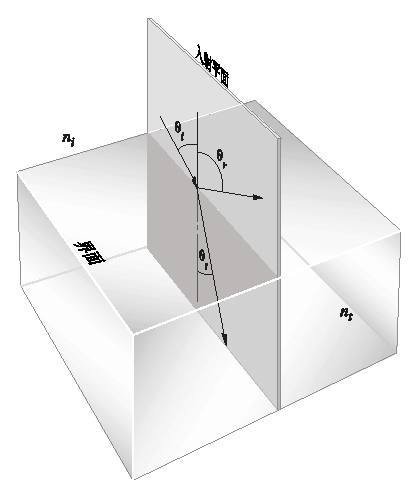
\includegraphics[width=0.5\linewidth]{chap06/ReflectionAndRefraction.eps}
    \caption{反射与折射分别遵循反射定律和折射定律。}
    \label{fig:6.26}
\end{figure}

\begin{proposition}
    \keyindex{反射定律}{law of reflection}{}:反射光线在入射平面内;
    反射光线和入射光线分居界面法线两侧;反射角等于入射角,即
    \begin{align}
        \theta_r=\theta_i \, .
    \end{align}
\end{proposition}
\begin{proposition}
    \keyindex{折射定律}{law of refraction}{}:折射光线在入射平面内;
    折射光线和入射光线分居界面法线两侧;折射角与入射角遵循\keyindex{斯涅尔定律}{Snell's law}{},即
    \begin{align}
        n_i\sin\theta_i=n_t\sin\theta_t \, .
    \end{align}
\end{proposition}
\begin{corollary}
    光线进入更大折射率的介质时会更偏向界面法线,
    进入更小折射率介质时则会更偏离法线。
\end{corollary}
\begin{definition}
    两种介质的绝对折射率之比定义为\keyindex{相对折射率}{relative index of refraction}{index of refraction折射率}:
    \begin{align}
        n_{ti}=\frac{n_t}{n_i}\, .
    \end{align}
    由此斯涅尔定律也可写作:
    \begin{align}
        \frac{sin\theta_i}{\sin\theta_t}=n_{ti}\, .
    \end{align}
\end{definition}

我们考虑\reffig{6.27}的情景:一束光线从点$S$起依次穿过$m$层介质并发生折射,
最终到达点$P$。设在每种介质中传播时对应的介质绝对折射率、路程、传播速度
分别为$n_j, s_j, v_j (j=1,\ldots,m)$。于是光线传播的总时间为
\begin{align}
    t=\sum\limits_{j=1}^{m}{\frac{s_j}{v_j}}\, ,
\end{align}
利用绝对折射率的定义可得
\begin{align}
    t=\frac{1}{c}\sum\limits_{j=1}^{m}{n_js_j}\, .
\end{align}
相对于空间路程$\sum\limits_{j=1}^{m}{s_j}$,
我们定义上式中的$\sum\limits_{j=1}^{m}{n_js_j}$
为\keyindex{光程}{optical path length}{}(OPL)。
更一般地,在非均匀介质中折射率是位置的函数,因此有
\begin{align}
    OPL=\int_S^P {n(s)\mathrm{d}s}\, .
\end{align}
\begin{figure}[htbp]
    \centering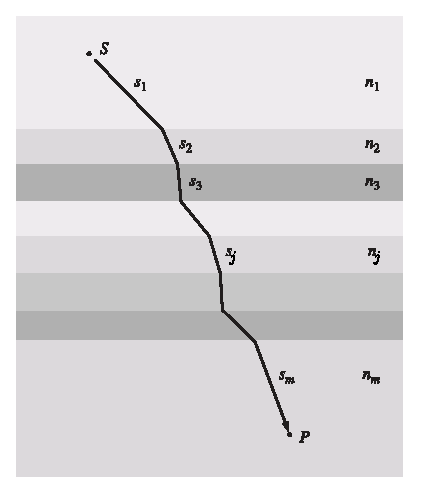
\includegraphics[width=0.5\linewidth]{chap06/PropagatingThroughLayeredMaterial.eps}
    \caption{在多层介质中传播的光线。}
    \label{fig:6.27}
\end{figure}

事实上,包括反射与折射在内,光的一般传播规律遵循费马原理。
它可推导出光线在真空中沿直线传播的性质以及反射定律和折射定律。
\begin{proposition}
    \keyindex{费马原理}{Fermat's principle}{}的现代形式是:
    光线从点$S$到点$P$的传播路径一定是对光程\keyindex{稳定}{stationary}{}的。
\end{proposition}

\begin{figure}[htbp]
    \centering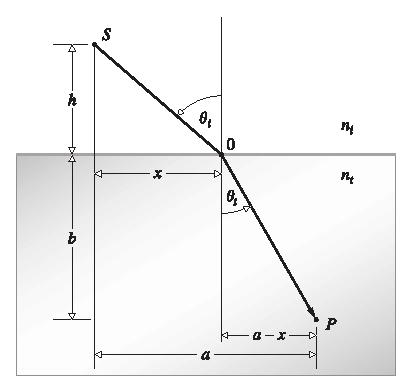
\includegraphics[width=0.5\linewidth]{chap06/FermatsPrincipleAppliedToRefraction.eps}
    \caption{费马原理运用于折射。}
    \label{fig:6.28}
\end{figure}

如\reffig{6.28}所示,我们利用费马原理来推导斯涅尔定律:
\begin{prove}
    考虑从点$S$到点$P$的光线,它在界面上点$O$处发生折射,
    相应量已标在途中图中。其光程为
    \begin{align}
        OPL=n_i\overline{SO}+n_t\overline{OP}=n_i\sqrt{x^2+h^2}+n_t\sqrt{b^2+(a-x)^2}\, .
    \end{align}

    依据费马原理,我们令$\displaystyle\frac{\mathrm{d}OPL}{\mathrm{d}x}=0$,可得
    \begin{align}
        \frac{n_ix}{\sqrt{x^2+h^2}}-\frac{n_t(a-x)}{\sqrt{b^2+(a-x)^2}}=0\, .
    \end{align}
    注意到$\displaystyle\sin\theta_i=\frac{x}{\sqrt{x^2+h^2}}$以及
    $\displaystyle\sin\theta_t=\frac{(a-x)}{\sqrt{b^2+(a-x)^2}}$,带入得
    \begin{align}
        n_i\sin\theta_i=n_t\sin\theta_t\, .
    \end{align}
    即得到斯涅尔定律。
\end{prove}

\begin{figure}[htbp]
    \centering
    \subfloat[日常的反射光可视作由无数原子级散射复合而成,例如这张人脸。]
    {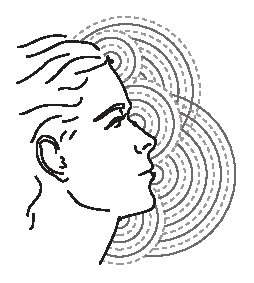
\includegraphics[width=0.25\linewidth]{chap06/PersonFace.eps}\label{fig:6.29.1}}\,
    \subfloat[光学系统的共轭点]{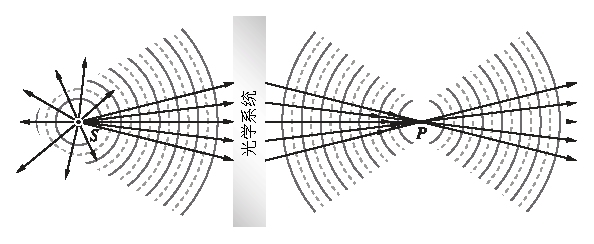
\includegraphics[width=0.7\linewidth]{chap06/ConjugateFoci.eps}\label{fig:6.29.2}}
    \caption{光的发散与汇聚。}
    \label{fig:6.29}
\end{figure}

如\reffig{6.29.1},自身发光或被照亮的物体可以视作是大量辐射点\keyindex{源}{source}{}构成的。
每个点源都在发出\keyindex{球面波}{spherical wave}{}。
此时我们说光线从给定点源\keyindex{发散}{diverge}{}。
反之,若球面波坍缩到一点,我们说光线\keyindex{汇聚}{converge}{}到该点。
实际中我们往往只处理\keyindex{波前}{wavefront}{}的一部分。
在\keyindex{几何光学}{geometrical optics}{optics光学}中,
我们研究如何通过插入反射和折射体来控制改变波前(光线)并忽略所有衍射效应。
如\reffig{6.29.2}所示,当点$S$发散的一部分波前经过\keyindex{光学系统}{optical system}{}后
汇聚到点$P$时,依据光路可逆性原理,在点$P$处发散的波前可以反向经过该系统处理后汇聚到点$S$。
我们称点$S$和点$P$互为\keyindex{共轭点}{conjugate point}{}。
对于理想光学系统,三维空间中的任意区域都会完美成像为另一区域,
前者称为\keyindex{物空间}{object space}{},后者称为\keyindex{像空间}{image space}{}。

\subsection{透镜}\label{sub:透镜}
\begin{definition}
    \keyindex{透镜}{lens}{}是重新配置能量传播分布的折射器件,
    即意味着现有介质的不连续性。
\end{definition}

如\reffig{6.30},最常见的是中间厚边缘薄的\keyindex{凸透镜}{convex lens}{lens透镜},
也称\keyindex{汇聚透镜}{converging lens}{lens透镜}、\keyindex{正透镜}{positive lens}{lens透镜},
以及中间薄边缘厚的\keyindex{凹透镜}{concave lens}{lens透镜},
也称\keyindex{发散透镜}{diverging lens}{lens透镜}、\keyindex{负透镜}{negative lens}{lens透镜}。
当一束平行光穿过凸透镜(或凹透镜)时,
光线汇聚的点(或从之发散的点)称为透镜的一个\keyindex{焦点}{focal point}{}。
对于\reffig{6.30}(b),将点源置于透镜前方光轴上的$F_1$处,光线汇聚到共轭点$F_2$。
此时若在$F_2$处放置一个光屏,则屏上会有相应发亮的像,称该像是\keyindex{实}{real}{}的。
对于\reffig{6.30}(c),将点源置于透镜前方无穷远处,从透镜射出的光是发散的,
且看起来好像是从点$F_2$发散。但在该位置的光屏上不会出现发亮的像,所以称该像是\keyindex{虚}{virtual}{}的。
\begin{figure}[htbp]
    \centering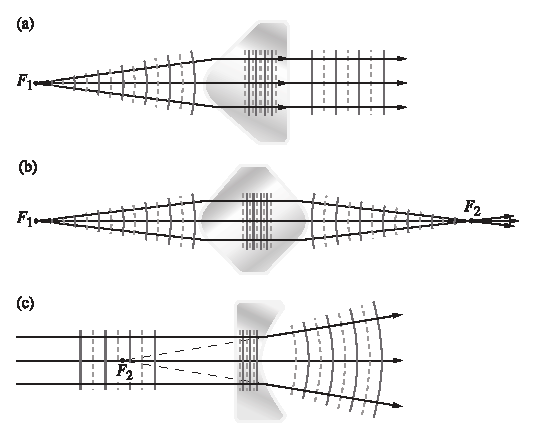
\includegraphics[width=0.8\linewidth]{chap06/HyperbolicLenses.eps}
    \caption{几种双曲面透镜横截面。其中(a)和(b)是凸透镜,(c)是凹透镜。}
    \label{fig:6.30}
\end{figure}

\subsubsection{球面透镜的折射}
现实生活中绝大多数透镜的表面是一片球面,因为它的制造难度比非球面透镜低得多。
尽管这种透镜会有\keyindex{像差}{aberration}{},但现代制造技术可以把它控制在极小范围内。
以下我们将探讨球面透镜的成像规律,并约定后文中的透镜都是关于光轴旋转对称的。
\begin{figure}[htbp]
    \centering
    \subfloat[球形界面上的折射。]{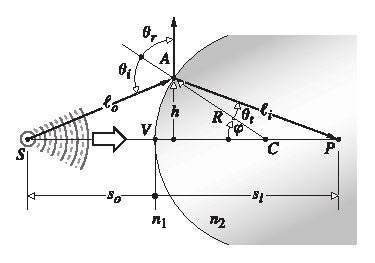
\includegraphics[width=0.48\linewidth]{chap06/RefractionSphericalInterface.eps}\label{fig:6.31.1}}\,
    \subfloat[球形界面上相同入射角的光线。]{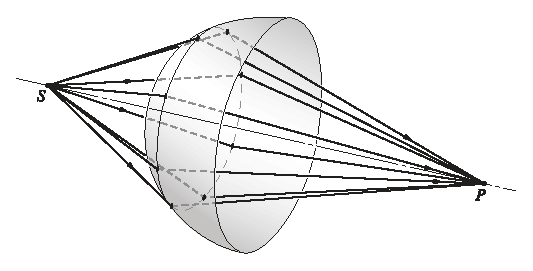
\includegraphics[width=0.5\linewidth]{chap06/IncidentSameAngle.eps}\label{fig:6.31.2}}
    \caption{球面透镜的折射。}
    \label{fig:6.31}
\end{figure}

\reffig{6.31}展示了位于点$S$处的点源发出的波遇到
以点$C$为中心且半径为$R$的球面透镜界面后的折射情况。
外部介质和透镜的折射率分别为$n_1$和$n_2 (n_1<n_2)$。
点$V$称为界面的\keyindex{顶点}{vertex}{}。
长度$s_o=\overline{SV}$称为\keyindex{物距}{object distance}{}。
光线$\overline{SA}$在界面上点$A$发生折射后偏向局部法线,也偏向了光轴,
设于光轴交于点$P$,入射角为$\theta_i$,折射角为$\theta_t$。
注意最终过点$P$的折射光线都有相同的入射角(\reffig{6.31.2})。
长度$s_i=\overline{VP}$称为\keyindex{像距}{image distance}{}。
连线$\overline{CA}$与光轴的夹角为$\varphi$,并记
长度$\mathcal{l}_o=\overline{SA}, \mathcal{l}_i=\overline{AP}$。
因此光线从点$S$经$A$到$P$的光程为
\begin{align}
    OPL=n_1\mathcal{l}_o+n_2\mathcal{l}_i\, ,
\end{align}
其中$\mathcal{l}_o$和$\mathcal{l}_i$可分别在$\triangle SAC$和$\triangle ACP$中应用余弦定理得到:
\begin{align}
    \mathcal{l}_o & =\sqrt{R^2+(s_o+R)^2-2R(s_o+R)\cos\varphi}\, ,       \\
    \mathcal{l}_i & =\sqrt{R^2+(s_i-R)^2-2R(s_i-R)\cos(\pi-\varphi)}\, .
\end{align}

考虑到点$A$的位置由$\varphi$完全决定,而$n_1, n_2, s_o, s_i, R$等量是定值,
所以光程是关于$\varphi$的函数。
依据费马原理,令光程对$\varphi$的导数为零,得到
\begin{align}
    \frac{n_1R(s_o+R)\sin\varphi}{\mathcal{l}_o}-\frac{n_2R(s_i-R)\sin\varphi}{\mathcal{l}_i}=0\, ,
\end{align}
整理后为
\begin{align}
    \frac{n_1}{\mathcal{l}_o}+\frac{n_2}{\mathcal{l}_i}=\frac{1}{R}\left(\frac{n_2s_i}{\mathcal{l}_i}-\frac{n_1s_o}{\mathcal{l}_o}\right)\, .
\end{align}

也就是说,从点$S$到点$P$的折射光线必定遵循上述数量规律。
事实上该规律不要求$s_o$等量必须为正数。具体来说:
\begin{itemize}
    \item 当点$S$在点$V$左边时,$s_o$取正,反之取负;
    \item 当点$P$在点$V$右边时,$s_i$取正,反之取负;
    \item 当点$C$在点$V$右边时,$R$取正,反之取负。
\end{itemize}

按照这样的约定确定符号时,该规律对球面凹透镜同样适用。
然而它形式仍较复杂,我们考虑进一步化简它:当$\varphi$非常接近0时,点$A$十分接近点$V$,
且此时运用一阶近似$\sin\varphi\approx\varphi$和$\cos\varphi\approx 1$易
知$\mathcal{l}_o\approx s_o, \mathcal{l}_i\approx s_i$,此时近似有
\begin{align}\label{eq:6.24}
    \frac{n_1}{s_o}+\frac{n_2}{s_i}=\frac{n_2-n_1}{R}\, ,
\end{align}

我们称这样与光轴所成角度很小的光线为\keyindex{近轴光线}{paraxial ray}{ray光线}。
注意\refeq{6.24}在关于光轴对称的很小一片区域上与点$A$的位置无关,
我们称该区域为\keyindex{近轴区域}{paraxial region}{}。
1841年,高斯在上述近似下系统阐述了成像规律,因此也称该结论为
一阶、近轴或\keyindex{高斯光学}{Gaussian optics}{optics光学}。

如\reffig{6.32.1},当光轴上点$F_o$的像在无穷远时,$s_i=\infty$,此时的物距$s_o$称为
\keyindex{第一焦距}{first focal length}{focal length焦距}或
\keyindex{物焦距}{object focal length}{focal length焦距}$f_o$,即
\begin{align}
    f_o=\frac{n_1}{n_2-n_1}R\, .
\end{align}
点$F_o$称为\keyindex{第一焦点}{first focus}{focus焦点}或\keyindex{物焦点}{object focus}{focus焦点}。
当$f_o>0$时,焦点$F_o$在顶点$V$左侧,反之在右侧。
类似地如\reffig{6.32.2},当$s_o=\infty$时,光轴上对应成像的点$F_i$
称为\keyindex{第二焦点}{second focus}{focus焦点}或\keyindex{像焦点}{image focus}{focus焦点}。
此时的像距$s_i$称为\keyindex{第二焦距}{second focal length}{focal length焦距}或\keyindex{像焦距}{image focal length}{focal length焦距},即
\begin{align}
    f_i=\frac{n_2}{n_2-n_1}R\, .
\end{align}
且当$f_i>0$时,焦点$F_i$在顶点$V$右侧,反之在左侧。
\begin{figure}[htbp]
    \centering
    \subfloat[物焦点与物焦距]{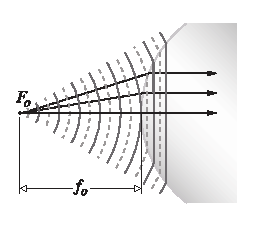
\includegraphics[width=0.4\linewidth]{chap06/ObjectFocus.eps}\label{fig:6.32.1}}\,\,
    \subfloat[像焦点与像焦距]{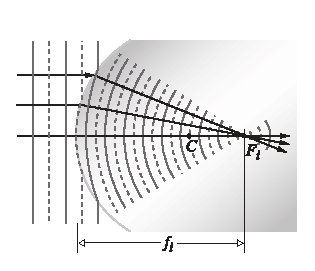
\includegraphics[width=0.45\linewidth]{chap06/ImageFocus.eps}\label{fig:6.32.2}}
    \caption{球面透镜的焦距与焦点}
    \label{fig:6.32}
\end{figure}

之前我们说过,当出射光线是发散时我们称该像是虚的(\reffig{6.33.1}),
此时$s_i<0$,像点$F_i$在顶点$V$的左边;类似地,当入射光线是汇聚时我们称物是虚的
(\reffig{6.33.2}),此时$s_o<0$,物点$F_o$在顶点$V$右边。
\begin{figure}[htbp]
    \centering
    \subfloat[虚像点]{\vspace{-5cm}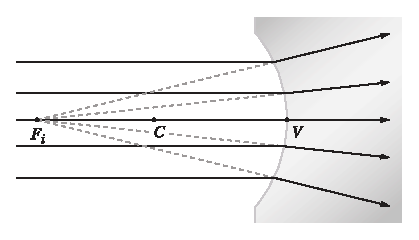
\includegraphics[width=0.5\linewidth]{chap06/VirtualImagePoint.eps}\label{fig:6.33.1}}\,\,\,
    \subfloat[虚物点]{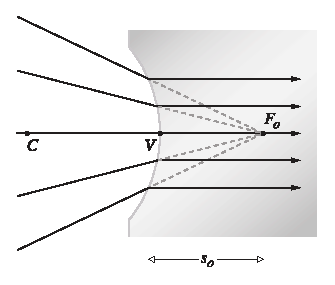
\includegraphics[width=0.4\linewidth]{chap06/VirtualObjectPoint.eps}\label{fig:6.33.2}}
    \caption{虚像点和虚物点}
    \label{fig:6.33}
\end{figure}

\subsubsection{薄透镜}
只有一个元件(即两个折射界面)的称为\keyindex{简单透镜}{simple lens}{lens透镜},
多于一个元件的称为\keyindex{复合透镜}{compound lens}{lens透镜}。
此外按照透镜厚度能否忽略还可以分为\keyindex{薄透镜}{thin lens}{lens透镜}和\keyindex{厚透镜}{thick lens}{lens透镜}。
以下我们讨论简单薄透镜的成像规律。
\begin{figure}[htbp]
    \centering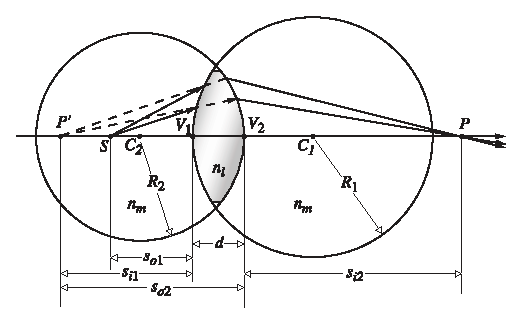
\includegraphics[width=0.75\linewidth]{chap06/SphericalLens.eps}
    \caption{球面透镜的成像规律}
    \label{fig:6.34}
\end{figure}

\reffig{6.34}展示了两个界面都是球面的透镜是如何折射光线的。
这里外部介质折射率为$n_m$,透镜折射率为$n_l, (n_l>n_m)$,
左边(第一)界面的球心为$C_1$,半径为$R_1>0$,顶点为$V_1$;
右边(第二)界面的球心为$C_2$,半径为$R_2<0$,顶点为$V_2$。
两个顶点距离为$d$。在近轴近似下,光轴上的点源$S$发出的光线经过
第一界面折射后的像点为$P'$,对应有物距$s_{o1}=\overline{SV_1}>0$,
像距$s_{i1}=\overline{V_1P'}<0$;
同时$P'$也是第二次折射的物点,折射后为光轴上的像点$P$,
并有物距$s_{o2}=\overline{P'V_2}>0$,像距$s_{i2}=\overline{V_2P}>0$。
根据\refeq{6.24}的结论,两次折射分别满足:
\begin{align}
    \frac{n_m}{s_{o1}}+\frac{n_l}{s_{i1}} & =\frac{n_l-n_m}{R_1}\, , \\
    \frac{n_l}{s_{o2}}+\frac{n_m}{s_{i2}} & =\frac{n_m-n_l}{R_2}\, .
\end{align}
考虑到$|s_{o2}|=|s_{i1}|+d$,结合各量正负性带入上式整理得
\begin{align}
    \frac{n_m}{s_{o1}}+\frac{n_m}{s_{i2}}=(n_l-n_m)\left(\frac{1}{R_1}-\frac{1}{R_2}\right)+\frac{n_ld}{(s_{i1}-d)s_{i1}}\, .
\end{align}
注意到对于整个透镜而言,其物距为$s_o=s_{o1}$,像距为$s_i=s_{i2}$。
当透镜很薄时,$d\approx 0$,点$V_1$和$V_2$十分靠近,所以上式右边最后一项可以舍去。
同时假设外部介质是空气,即$n_m\approx 1$,
于是我们得到:
\begin{proposition}
    \keyindex{薄透镜方程}{thin-lens equation}{}:
    \begin{align}
        \frac{1}{s_o}+\frac{1}{s_i}=(n_l-1)\left(\frac{1}{R_1}-\frac{1}{R_2}\right)\, .
    \end{align}
\end{proposition}

事实上该结论对各量取正负的情况都成立。分别令物距和像距取无穷远,
可以得到透镜对应的像焦距$f_i=\lim\limits_{s_o\to\infty}s_i$
和物焦距$f_o=\lim\limits_{s_i\to\infty}s_o$。
显然$f_i=f_o$,我们去掉下标把焦距记为$f$,则有
\begin{align}
    \frac{1}{f}=(n_l-1)\left(\frac{1}{R_1}-\frac{1}{R_2}\right)\, .
\end{align}
由此得到
\begin{proposition}
    \keyindex{高斯透镜公式}{Gaussian lens formula}{}:
    \begin{align}
        \frac{1}{s_o}+\frac{1}{s_i}=\frac{1}{f}\, .
    \end{align}
\end{proposition}

\begin{figure}[htbp]
    \centering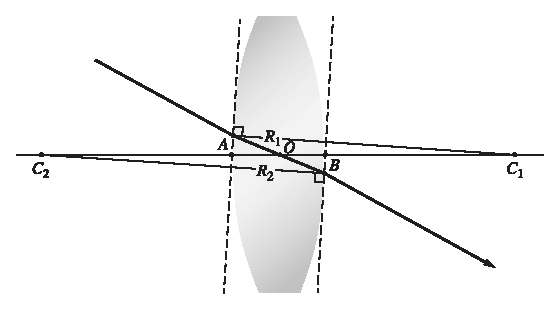
\includegraphics[width=0.75\linewidth]{chap06/OpticalCenter.eps}
    \caption{球面透镜的光心}
    \label{fig:6.35}
\end{figure}

对于球面透镜而言,过光心的光线不改变传播方向。
如\reffig{6.35}所示,我们取一对平行平面分别与两界面相切于点$A$和点$B$。
分别过点$A$和点$B$作平面的垂线,由于这是球面透镜,它们必和光轴交于
对应球心$C_1$和$C_2$,于是$AC_1$平行于$BC_2$,且易知$A, B, C_1, C_2$四点共面。
设$AB$与$C_1C_2$交于点$O$,则有$\triangle AOC_1\sim\triangle BOC_2$,于是
\begin{align}
    \frac{|R_1|}{|R_2|}=\frac{\overline{OC_1}}{\overline{OC_2}}\, .
\end{align}
考虑到$R_1, R_2, \overline{C_1C_2}$均为定值,所以$O$是定点。
又因为$\angle OAC_1=\angle OBC_2$,所以第一界面的折射角等于第二界面的入射角,
两次折射介质相反,所以第一界面的入射角等于第二界面的折射角,即入射光线与最终出射光线同向。
也就是说,当且仅当光线经过球面透镜的定点$O$时不改变方向,称定点$O$为透镜的\keyindex{光心}{optical center}{}。
此时光线的横向偏移量正比于透镜厚度。对于薄透镜而言,我们可以近似地把整条过光心的光线视作直线。

我们已经知道平行近轴光线会被球形界面聚焦到一点。
因此如\reffig{6.36}所示,若干束与光轴倾角很小、范围很小、且垂直于界面入射的光线
对应的焦点将分布在球面$\sigma$上,其球心即界面的球心$C$。
在光线范围很小的情况下,我们可把$\sigma$视作与透镜光轴垂直的平面,
称之为\keyindex{焦平面}{focal plane}{}。
如\reffig{6.37},在近轴假设下,所有平行光束都会被球面透镜聚焦
到\keyindex{第二焦平面}{second focal plane}{focal plane焦平面}上,
也称\keyindex{后焦平面}{back focal plane}{focal plane焦平面}。
类似地还有与物焦点对应的\keyindex{第一焦平面}{first focal plane}{focal plane焦平面},
也称\keyindex{前焦平面}{front focal plane}{focal plane焦平面}。
\begin{figure}[htbp]
    \centering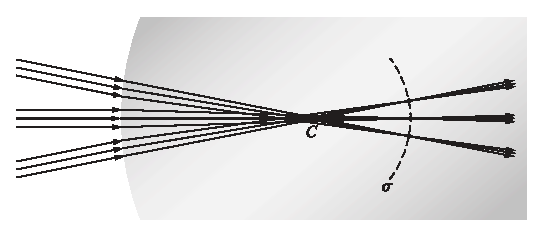
\includegraphics[width=0.75\linewidth]{chap06/FocusingSeveralRayBundles.eps}
    \caption{几束窄范围平行光的聚焦。}
    \label{fig:6.36}
\end{figure}
\begin{figure}[htbp]
    \centering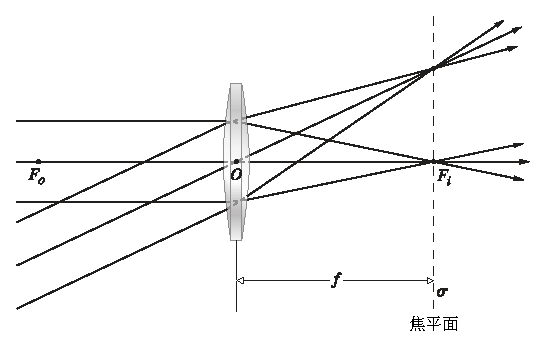
\includegraphics[width=0.75\linewidth]{chap06/FocalPlane.eps}
    \caption{透镜的焦平面。}
    \label{fig:6.37}
\end{figure}

对于透镜有三种特殊光线(包括延长线)帮助我们确定成像情况。
如\reffig{6.38}所示,它们分别是过光心而不改变方向的光线1、
平行于光轴入射而过焦点的光线2、过焦点入射而平行于光轴出射的光线3。
出射光线的交点即定出成像的位置、大小、倒立情况。
\begin{figure}[htbp]
    \centering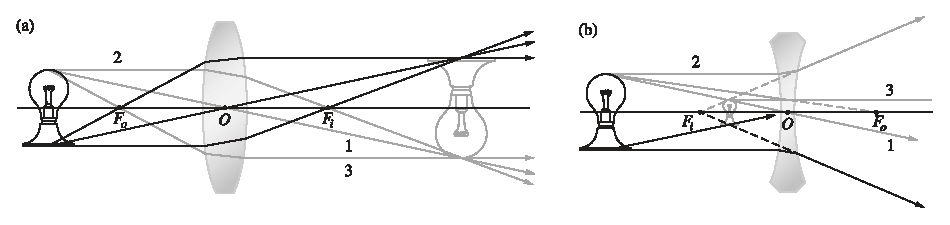
\includegraphics[width=\linewidth]{chap06/RealObjectAndPositiveLensAndNegativeLens.eps}
    \caption{利用三种特殊光线确定凸透镜和凹透镜对实物的成像。}
    \label{fig:6.38}
\end{figure}

我们接下来讨论薄透镜的具体成像规律。如\reffig{6.39}所示,
以焦距为$f$的凸透镜为例。分别记物和像偏移光轴的横向
\sidenote{横向指垂直于光轴的方向,下同。}距离为$y_o, y_i$,
在轴上方取正,下方取负。所以这里图中有$y_o>0, y_i<0$。
当$y_o$与$y_i$异号时,我们说像是\keyindex{倒}{inverted}{}的,
反之则是\keyindex{正}{erect}{}的。
记物到物焦点$F_o$的轴向距离为$x_o=\overline{S_1F_o}=s_o-f$,
当$S_1$在$F_o$左边时$x_o$取正,反之取负;
记像到像焦点$F_i$的轴向距离为$x_i=\overline{F_iP_1}=s_i-f$,
当$P_1$在$F_i$右边时$x_i$取正,反之取负。
\begin{figure}[htbp]
    \centering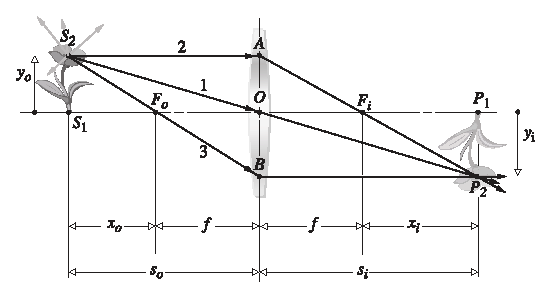
\includegraphics[width=0.75\linewidth]{chap06/ObjectAndImageLocation.eps}
    \caption{薄透镜成像时物和像的位置。}
    \label{fig:6.39}
\end{figure}

因为易知$\triangle AF_iO\sim\triangle P_2F_iP_1$,所以有
\begin{align}
    \frac{y_o}{|y_i|}=\frac{f}{x_i}\, .
\end{align}
类似地,因为$\triangle S_1F_oS_2\sim\triangle OF_oB$,所以有
\begin{align}
    \frac{y_o}{|y_i|}=\frac{x_o}{f}\, .
\end{align}
结合上面两式得到
\begin{proposition}
    薄透镜方程的\keyindex{牛顿形式}{Newtonian form}{}:
    \begin{align}
        x_ox_i=f^2\, .
    \end{align}
\end{proposition}
1704年牛顿首次在他的《Opticks》一书中阐述了该规律。
上式还说明,$x_o$与$x_i$一定同号,因此有
\begin{corollary}
    物和像一定在各自相应焦点的对侧。
\end{corollary}

\begin{definition}
    光学系统最终成像的横向维度与物的对应维度之比
    称为\keyindex{横向放大率}{transverse magnification}{},记作
    \begin{align}
        M_T=\frac{y_i}{y_o}\, .
    \end{align}
\end{definition}
不难发现,横向放大率还满足
\begin{align}
    M_T=-\frac{s_i}{s_o}=-\frac{x_i}{f}=-\frac{f}{x_o}\, .
\end{align}

\begin{corollary}
    $M_T>0$对应正像,$M_T<0$对应倒像。
\end{corollary}
\begin{corollary}
    单个薄透镜元件所成实像必是倒像。
\end{corollary}

\reftab{6.2}列出了薄透镜成像的规律,其中凸透镜部分与\reffig{6.40}对应。
\begin{table}[htbp]
    \centering
    \begin{tabular}{c|c|cccc}
        \toprule
        \multirow{2}{*}{\textbf{透镜类型}} & \multirow{2}{*}{\textbf{实物位置}} & \multicolumn{4}{c}{\textbf{像}}                                                                \\
        \cline{3-6}
                                           &                                    & \textbf{类型}                   & \textbf{位置}            & \textbf{朝向} & \textbf{相对大小} \\
        \midrule
        \multirow{5}{*}{凸透镜}            & $\infty>s_o>2f$                    & 实                              & $f<s_i<2f$               & 倒            & 缩小              \\
                                           & $s_o=2f$                           & 实                              & $s_i=2f$                 & 倒            & 相等              \\
                                           & $f<s_o<2f$                         & 实                              & $\infty>s_i>2f$          & 倒            & 放大              \\
                                           & $s_o=f$                            & -                               & $\pm\infty$              & -             & -                 \\
                                           & $s_o<f$                            & 虚                              & $|s_i|>s_o$              & 正            & 放大              \\
        \midrule
        凹透镜                             & 任意                               & 虚                              & $|s_i|<|f|$且$|s_i|<s_o$ & 正            & 缩小              \\
        \bottomrule
    \end{tabular}
    \caption{薄透镜对实物的成像。}
    \label{tab:6.2}
\end{table}

\begin{figure}
    \centering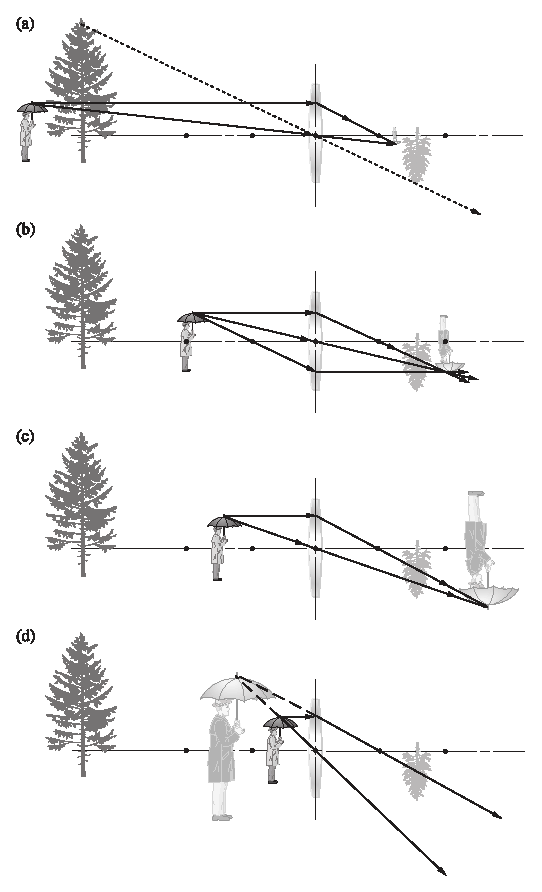
\includegraphics[width=0.75\linewidth]{chap06/ImageFormingBehavior.eps}
    \caption{薄凸透镜成像规律。}
    \label{fig:6.40}
\end{figure}